\chapter{System Design}

% \textit{Note: This chapter follows the System Design Document Template in \cite{bruegge2004object}. 
% You describe in this chapter how you map the concepts of the application domain to the solution domain. Some sections are optional, if they do not apply to your problem.
% Cite \cite{bruegge2004object} several times in this chapter.}

\section{Overview}

% \textit{Note: Provide a brief overview of the software architecture and references to other chapters (e.g. requirements analysis), references to existing systems, constraints impacting the software architecture.}

In this chapter, the decision regarding the architecture design of the application will be discussed.
Design of the architecture will be largely based on bridging the conceptual understanding of the application with the concrete technical solution.
Requirements of the system and existing constraints are also the main deciding factors of the architecture design.
The system also aims to address the nonfunctional requirements of the application, such as performance and usability, which were mentioned in earlier chapters.
Based on Bruegge and Dutoit's template \cite{bruegge2004object}, the structure of the system is divided into logical components and subsystems.

\section{Design Goals}

\textit{Note: Derive design goals from your nonfunctional requirements, prioritize them (as they might conflict with each other) and describe the rationale of your prioritization. Any trade-offs between design goals (e.g., build vs. buy, memory space vs. response time),
and the rationale behind the specific solution should be described in this section}

Design goals of the system are derived from nonfunctional requirements.
Because of constraints such as time, some of the nonfunctional requirements might not be fulfilled.

\begin{itemize} 
    \item \textbf{Usability and Accessibility}:
    One of the most important goal of the system is to be usable and accessible for the elderly.
    For this goal, the application is designed to be user-friendly for all age groups, specifically the elderly.
    The UI should be intuitive and easy to use.
    This is achieved through big buttons, clear visual indicators and enough spacing between elements.
    Design of the application should be accessible for the elderly with features such as large fonts, enough spacing, and clear visual indicators. 
    This design goal is purely achieved through the frontend of the application.
    As such, the only limiting constraint is the time and resources available to develop the frontend.

    \item \textbf{Reliability}: 
    Another most important goal of the system is reliability of the system.
    Reliability here means that the system should be able to accurately gather, process and store the typing pattern data.
    Since a faulty or inaccurate data could lead to wrong conclusion, the system should be able to minimize the inaccuracy of the data.
    Both the frontend and backend of the application play a role in achieving this goal.
    The frontend should be able to accurately capture the typing pattern data, especially the attribute timeSinceLastKey.
    This attribute shows information about the time difference between the last key press and the current key press.
    For this purpose, the built in JavaScript function Date.now() is used.

    \item \textbf{Performance}: 
    Recording the typing pattern data in real-time is not a performance heavy task.
    This function can easily be achieved by creating an array of keystroke data that is updated every time a key is pressed.
    The main performance issue of the application is waiting for the \ac{LLM} to respond to the user's message.
    The \ac{LLM} is instructed to try to get as much response from the users as possible, so that more typing data can be collected.
    This leads to a longer waiting time for the user to get a response, since the longer the response from the \ac{LLM}, the longer it will take for the \ac{LLM} to finish the response.
    One of the possibility of solving this problem would be to stream the response from the \ac{LLM}.
    Stream will allow the user to see response from the \ac{LLM} in chunks, instead of waiting for the whole response to be finished.
    Unfortunately this feature is not yet implemented in this application due to time constraints.

    \item \textbf{Privacy}: 
    An application that concerns itself with collecting sensitive user data should be secure and able to keep the data private.
    In this application, a chat session can be accessed by inputting a session ID.
    As a measure to increase privacy, each chat session can be made inaccessible by changing an attribute in the database.
    When a user tries to access a chat session that is already closed, the application will return an error message.
    Another important factor regarding privacy is anonimity.
    The only information about the user that is saved in the database is the user's age.
    If another user tries to access chat session of another user that is not yet deactivated, the message history will be shown.
    However, the user's age will not be shown.

    \item \textbf{Adaptability}: 
    Adaptability means the ease with which a system may be modified to fit changed requirements or environment.
    Adaptability of the system can be divided into two parts: adaptability of the frontend and adaptability of the backend.
    The frontend of the application is designed to be easily modifiable by utilising component based design of the React library.
    Adaptability of the backend is ensured by utilising concepts such as encapsulation and modularity.
    The backend is divided into several classes, each responsible for a specific task.
    This allows for easy modification of the backend, since each class can be modified without affecting the other classes.
    The only limiting factor for adaptability is the time and resources available to modify the system.
    Docker is used to containerize the application, which allows for easy deployment and scaling of the application.

\end{itemize}
    

\section{Subsystem Decomposition}

% \textit{Note: Describe the architecture of your system by decomposing it into subsystems and the services provided by each subsystem. Use UML class diagrams including packages / components for each subsystem.}

The system is divided into two main subsystems: the frontend and the backend.
The frontend is responsible for capturing the typing pattern data and displaying the chat interface.
The backend is responsible for processing the typing pattern data and generating a response from the \ac{LLM}.

\subsection{Frontend}

\subsubsection{User Interface}

\begin{figure}[h!]
    \centering
    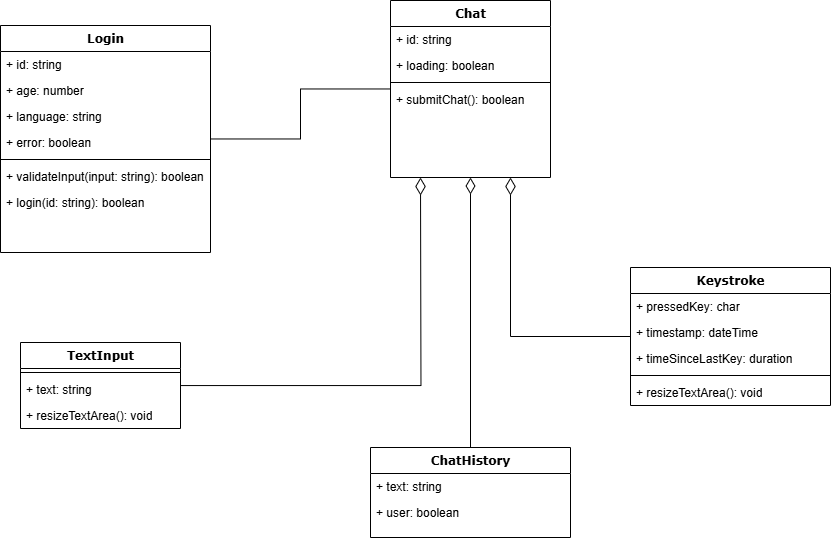
\includegraphics[width=13cm]{class_frontend.png}
    \caption{UML class diagram of the frontend architecture of the user interface}
    \label{class_frontend}
\end{figure}

The frontend of the application of the user interface can be divided into two main components: the login component and the chat component.
Figure~\ref{class_frontend} shows the UML class diagram of the frontend architecture of the user interface.
The main purpose of the login page is to initialise the chat session and validate the user's input.
User inputs their age, the session ID, and the language to chat with the \ac{LLM}.
English and german are the two possible languages that the user can choose.

In the login page, the user can click the "Login" button to start the chat.
After this button is clicked, both the session ID and the user's age will first be validated.
On the frontend side, the session ID is validated by checking whether the session ID has 6 digits.
The user's age is validated by checking whether the user's age is a number and whether the user's age is between 1 and 99.
If the validation is successful, the data will be sent to the backend.
On the backend side, the session ID is validated by checking whether the session ID is alredy deactivated.
The deactivated attribute is a boolean attribute in the database that can be managed either through the admin interface or by directly changing the value in the database.

\subsubsection{Admin Interface}

\begin{figure}[h!]
    \centering
    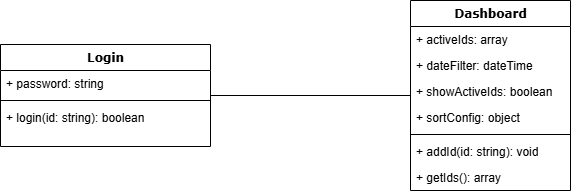
\includegraphics[width=13cm]{class_frontend_admin.png}
    \caption{UML class diagram of the frontend architecture of the admin interface}
    \label{class_frontend_admin}
\end{figure}

The admin interface is a separate component of the frontend that is only accessible by the admin.
Figure~\ref{class_frontend_admin} shows the UML class diagram of the frontend architecture of the admin interface.
This admin interface can also be divided into two main components: the login component and the dashboard component.
Login page of the admin interface is significantly simpler than the login page of the user interface.
The admin only needs to input the admin password to access the admin interface.
After the "Login" button is clicked, the inputted password will be checked against the password set in the backend of the application.

The dashboard component helps manage the chat sessions by providing these functionalities:
\begin{itemize}
    \item View the list of initialised chat sessions or initialised chat sessions that are still active
    \item Deactivate a chat session
    \item Initialise a new chat session by inputting the ID of the chat session
    \item Sort the chat sessions by added date, ID, or deactivated date to ease the process of finding a specific chat session
\end{itemize}

\subsection{Backend}

\subsubsection{Main Controller}

\begin{figure}[h!]
    \centering
    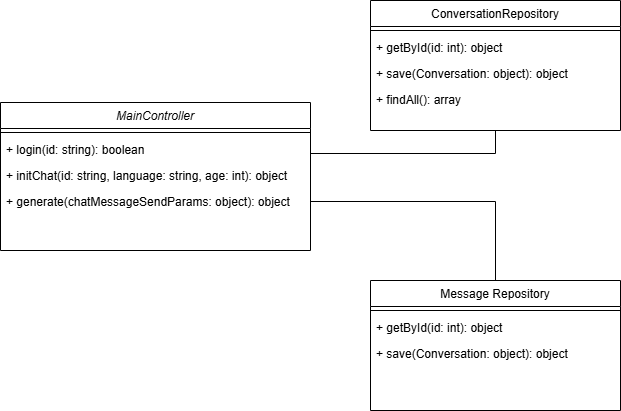
\includegraphics[width=13cm]{class_backend.png}
    \caption{UML class diagram of the backend architecture of the main controller}
    \label{class_backend}
\end{figure}

The backend of the application can be divided into two main components: main controller and admin controller.
Figure~\ref{class_backend} shows the UML class diagram of the main controller.
This controller is responsible for handling login, initialisation of a chat session and getting a response from the \ac{LLM}.

\subsubsection{Admin Controller}

\begin{figure}[h!]
    \centering
    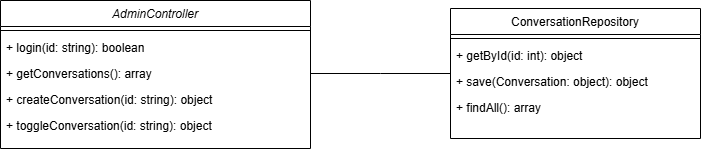
\includegraphics[width=13cm]{class_backend_admin.png}
    \caption{UML class diagram of the backend architecture of the admin controller}
    \label{class_backend_admin}
\end{figure}

Figure~\ref{class_backend_admin} shows the UML class diagram of the admin controller.
This controller is responsible for handling the admin login and managing the chat sessions.
For managing the chat sessions, this controller provides these functionalities: get all chat sessions, deactivate and reactivate a chat session, and initialise a new chat session.

% \section{Persistent Data Management}

% \textit{Note: Optional section that describes how data is saved over the lifetime of the system and which data.
%  Usually this is either done by saving data in structured files or in databases.
%  If this is applicable for the thesis, describe the approach for persisting data here and show a UML class diagram how the entity objects are mapped to persistent storage.

% It contains a rationale of the selected storage scheme, file system or database, a description of the selected database and database administration issues.
% }

% \section{Access Control}

% \textit{Note: Optional section describing the access control and security issues based on the nonfunctional requirements in the requirements analysis.
%  It also describes the implementation of the access matrix based on capabilities or access control lists, the selection of  authentication mechanisms and the use of encryption algorithms.
% }

% \section{Global Software Control}

% \textit{Note: Optional section describing describing the control flow of the system, in particular, whether a monolithic, event-driven control flow or concurrent processes have been selected, how requests are initiated and specific synchronization issues}


% \section{Boundary Conditions}

% \textit{Note: Optional section describing the use cases how to start up the separate components of the system, how to shut them down, and what to do if a component or the system fails.}
